\providecommand{\main}{..}
\documentclass[../COS3712_Notes.tex]{subfiles}

\begin{document}
  \setcounter{chapter}{6}
  \chapter{Discrete Techniques}
    \section{Buffers}
      What all buffers have in common is that they are inherently discrete:
      they have limited resolution, both spatially and in depth.
      We can define a (two-dimensional) \concept{buffer} as block of memory with
      $n \times m$ $k$-bit elements.

      The \concept{framebuffer} is the set of buffers that the graphics system uses for rendering,
      including the front and back colour buffers, the depth buffer, and other buffers
      the hardware may provide.

    \section{Mapping Methods}
      One of the most powerful uses of discrete data is for surface rendering.
      The process of modelling an object by a set of geometric primitives and then rendering
      these primitives has its limitations.

      An alternative is not to attempt to build increasingly more complex models,
      but rather to build a simple model and to add detail as part of the rendering process.
      As the implementation renders a surface, it generates a set of fragments,
      each of which corresponds to a pixel in the framebuffer.
      Fragments carry colour, depth, and other information that can be used to determine
      how they contribute to the pixels in which they correspond.
      As part of the rasterization process, we must assign a shade or colour to each fragment.
      These colours can be modified during fragment processing after rasterization.
      The mapping algorithms can be thought of as wither modifying the shading algorithm
      based on a 2D-array, the map, or modifying the shading by using the map to alter the
      surface using three major techniques:
      \begin{itemize}[nosep]
        \item Texture mapping
        \item Bump mapping
        \item Environment mapping
      \end{itemize}

      \begin{definition}{Texture Mapping}
        Uses an image (or texture) to influence the colour of a fragment.
        Textures can be specified using a fixed pattern; by a procedural texture generation
        method; or through a digitized image.
        In all cases, we can characterise the resulting image as the mapping of a texture
        to a surface, which is carried out as part of the rendering of the surface.
      \end{definition}

      \begin{definition}{Bump Maps}
        Unlike texture maps, which paint patterns onto smooth surfaces,
        \concept{bump~maps} distort the normal vectors during the shading process to make the
        surface appear to have small variations in shape.
      \end{definition}

      \begin{definition}{Environment Maps (Reflection Maps)}
        Allow us to create images that have the appearance of reflected materials
        without having to trace reflected rays.
        An image of the environment is painted onto the surface as that surface is being
        rendered.
      \end{definition}

      \begin{sidenote}{Similarities Between the Three Methods}
        $ $\vspace{-1em}
        \begin{itemize}[nosep]
          \item All three alter the shading of individual fragments as part of fragment processing.
          \item All rely on the map being stored as a one-, two-, or three-dimensional image.
          \item All keep the geometric complexity low while creating the illusion of complex
            geometry.
          \item All are subject to aliasing errors.
        \end{itemize}
      \end{sidenote}

      Two-dimensional texture mapping is supported by WebGL.
      Environment maps are a special case of standard texture mapping, but can be altered
      to create a variety of new effects in the fragment shader.
      Bump mapping requires us to process each fragment independently,
      something we can do with a fragment shader.

    \section{Two-Dimensional Texture Mapping}
      Textures are patterns, and can be one-, two-, three, or four-dimensional.
      Because the use of surfaces is so important in computer graphics,
      mapping 2D textures to surfaces is by far the most common use of texture mapping.

      Although there are multiple approaches to texture mapping, all require a sequence
      of steps that involve mappings around three or four different coordinate systems:
      \begin{descriptimize}[nosep]
        \item[Screen coordinates.] Where the final image is produced.
        \item[Object coordinates.] Where we describe the objects on which the textures will
          be mapped.
        \item[Texture coordinates.] Used to locate positions in the texture.
        \item[Parametric coordinates.] Used to specify parametric surfaces.
      \end{descriptimize}

      In most applications, textures start out as 2D images.
      These images are brought into processor memory as arrays.
      We call the elements of these arrays \concept{texels (texture elements)},
      rather than pixels, to emphasise how they will be used.
      We prefer to think of this array as a continuous rectangular two-dimensional texture pattern
      $T(s, t)$.
      The independent variables $s$ and $t$ are known as \concept{texture coordinates}.
      We can scale our texture coordinates to vary over the interval $[0.0, 1.0]$.

      A \concept{texture map} associates a texel with each point on a geometric object
      that is itself mapped to screen coordinates for display.

      One way to think about texture mapping is in terms of two concurrent mappings:
      the first from texture coordinates to object coordinates,
      and the second from parametric coordinates to object coordinates.
      A third mapping takes us from object coordinates to screen coordinates.

      Conceptually, the texture mapping process is simple.
      A small area of texture pattern maps to the area of the geometric surface,
      corresponding to a pixel in the final image.

    \section{Texture Mapping in WebGL}
      WebGL's texture maps rely on its pipeline architecture.
      There are two parallel pipelines: the geometric pipeline, and the pixel pipeline.
      For texture mapping, the pixel pipeline merges with fragment processing after rasterization.
      This architecture determines the type of texture mapping that is supported.
      Texture mapping is done as part of fragment processing.
      Each fragment that is generated can then be tested for visibility with the $z$-buffer.
      We can think of texture mapping as part of the shading process, but a part that is done
      on a fragment-by-fragment basis.

      Texture coordinates are handled like normals and colours:
      they can be associated with vertices as an additional vertex attribute,
      and the required texture values can be obtained by the rasterizer interpolating
      the texture coordinates at the vertices across polygons.
      They can also be generated in one of the shaders.

      \begin{figure}
        \begin{center}
          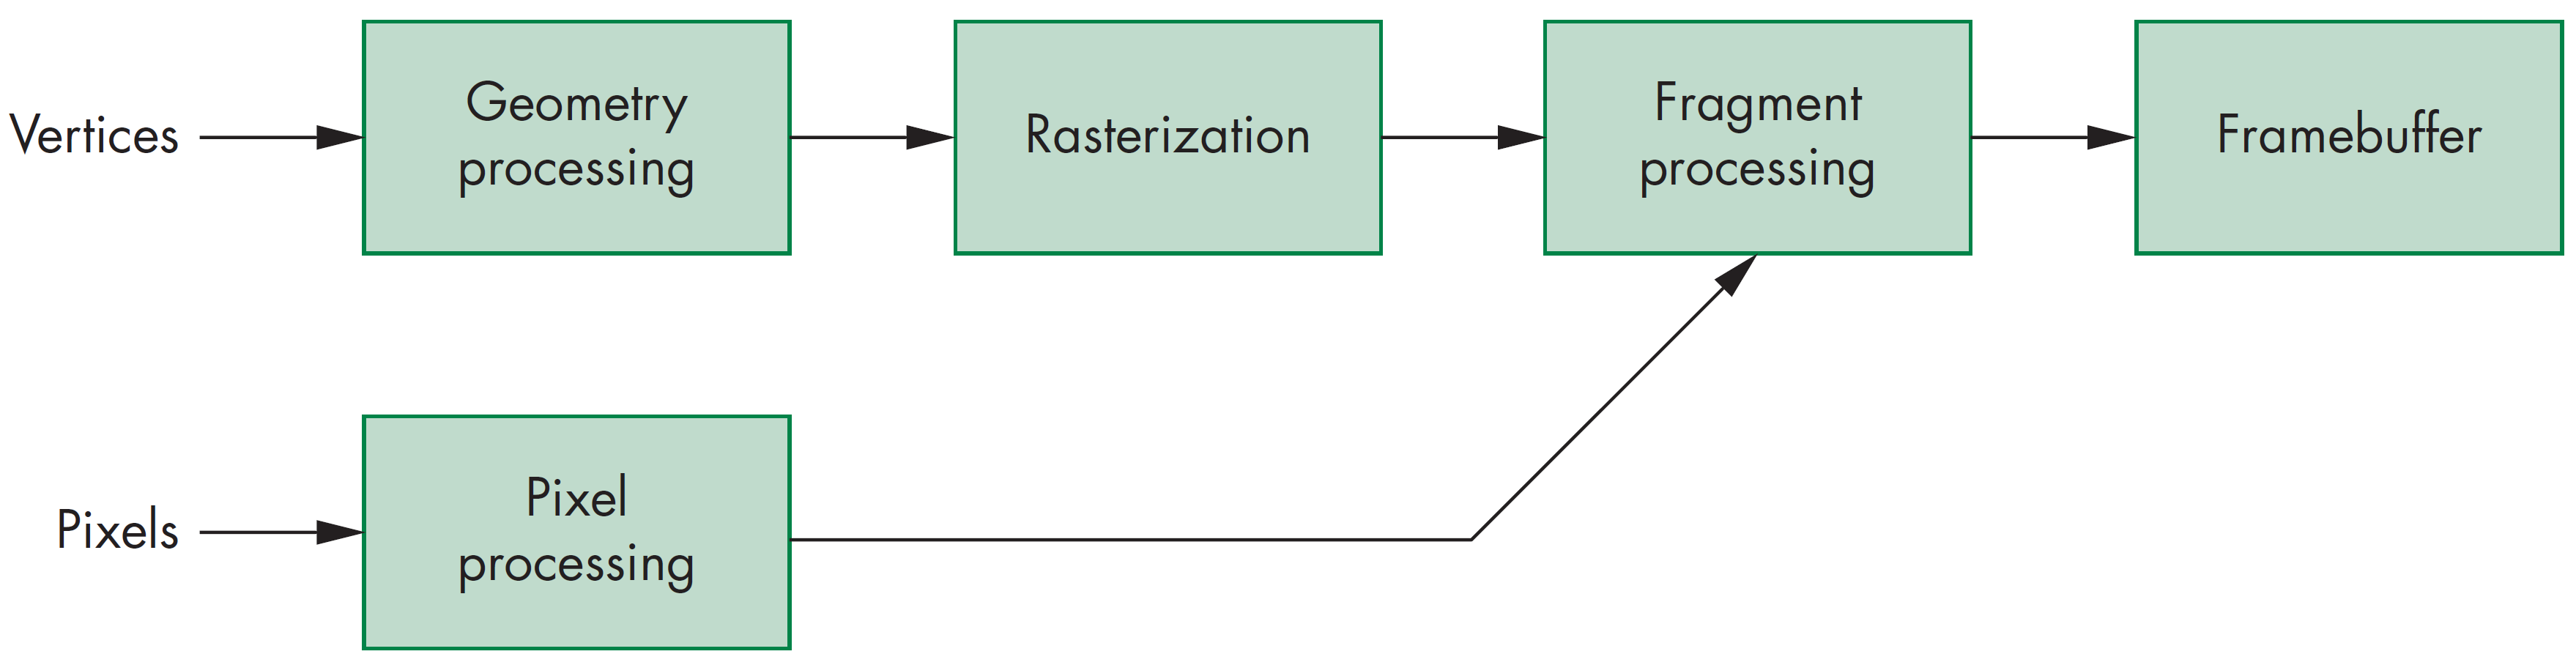
\includegraphics[width=0.8\textwidth]{\main/images/chapter07/two_pipelines.png}
        \end{center}
        \caption{Pixel and geometry pipelines.}
      \end{figure}

      Texture mapping requires interaction among the application program, the vertex shader,
      and the fragment shader.
      There are three basic steps:
      \begin{enumerate}
        \item Form a texture image and place it in texture memory on the GPU.
        \item Assign texture coordinates to each fragment.
        \item Apply the texture to each fragment.
      \end{enumerate}

      \subsection{Texture Objects}
        In early versions of OpenGL, there was only a single texture,
        the \concept{current texture}, that existed at any time.
        Each time a different texture was needed, we had to set up a new texture map.

        \concept{Texture~objects} allow the application program to define objects that consist
        of the texture array and the various texture parameters that control its application
        to surfaces.
        As long as there is sufficient memory to retain them, these objects reside in the
        texture memory in the GPU.

        \begin{sidenote}{Creating Textures}
          For a single texture, we start by creating a texture object:
          \begin{minted}[autogobble]{javascript}
            var texture = gl.createTexture();
          \end{minted}
          and then bind it as the current 2D texture object by executing
          \begin{minted}[autogobble]{javascript}
            gl.bindTexture(gl.TEXTURE_2D, texture);
          \end{minted}
          Subsequent texture function specify the texture image and its parameters,
          which become part of this texture object.
          We can delete an unused texture object with the function
          \mintinline{javascript}{gl.deleteTexture}.
        \end{sidenote}

      \subsection{Texture Coordinates and Samplers}
        The key element in applying a texture in the fragment shader is the mapping
        between the location of a fragment and the corresponding location within the texture image
        where we will get the texture colour for that fragment.
        Because each fragment has a location in the framebuffer that is one of its attributes,
        we need not refer to this position explicitly in the fragment shader.
        The potential difficulty is identifying the desired location in the texture image.

        We use two floating point texture coordinates, $s$ and $t$,
        both of which range over the interval $[0.0, 1.0]$ as we traverse the texture image.
        It is up to the application and the shaders to determine the appropriate texture
        coordinates for a fragment.
        The most common method is to treat texture coordinates as a vertex attribute.
        Thus, we could provide texture coordinates just as we provide vertex colours
        in the application.
        We would then pass these coordinates to the vertex shader and let the rasterizer
        interpolate the vertex texture coordinates to fragment texture coordinates.

        The vertex shader is only concerned with the texture coordinates,
        and has nothing to do with the texture object we created earlier.

        The key to putting everything together is a new type of variable called a \concept{sampler},
        which we usually only use in a fragment shader.
        A sampler variable provides access to a texture object, including all its parameters.
        There are two types of sampler variables for the types of textures supported in WebGL:
        \begin{itemize}
          \item the two-dimensional (\mintinline{javascript}{sampler2D}), and
          \item the cube map (\mintinline{javascript}{samplerCube}).
        \end{itemize}
        What a sampler does is return a value or sample of the texture image
        for the input texture coordinates.

      \subsection{Texture Sampling}
        Aliasing of textures is a major problem.
        When we map texture coordinates to the array of texels, we rarely get a point
        that corresponds to the centre of a texel.
        There are two options:
        \begin{descriptimize}
          \item[Point Sampling] Use the value of the texel that is closest to the texture
            coordinate output by the rasterizer.
            This option has the most visible aliasing errors.
          \item[Linear Filtering] Use a weighted average of a group of texels in the neighbourhood
            of the texel determined by point sampling.
            This strategy is better, but requires more work.
        \end{descriptimize}
        If we are using linear filtering, there is a problem at the edges of the texel array,
        because we need additional texel values outside the array.

        There is a further complication in deciding how to use the texel values to obtain
        a texture value: the size of the pixel we are trying to colour on the screen
        may be smaller or larger than one texel.
        In the first case, the texel is larger than one pixel (\concept{magnification});
        in the second, it is smaller (\concept{minification}).
        In both cases, the fastest strategy is to use the value of the nearest point sampling.

        WebGL has another way to deal with the minification problem: \concept{mipmapping}.
        For objects that project to an area of screen space that is small compared with the size
        of the texel array, we do not need the resolution of the original texel array.
        WebGL allows us to create a series of texture arrays at reduced sizes;
        it will then automatically use the appropriate size texture in this pyramid of textures,
        the one for which the size of the texel is approximately the size of a pixel.

\end{document}
